\subsection{Planificación de Implementación del Sistema}
En este plan se describirá cómo se llevará a cabo el despliegue del sistema, incluyendo publicidad, instalaciones , software, hardware y configuraciones.

Si bien ofrecemos una API pública y una interfaz web que facilita el uso a cualquier usuario, contemplamos que muchas de las instituciones necesitarán gestionar el sistema en un servidor propio. Por este motivo se ha desarrollado dicho documento que permitirá llevar a cabo de manera adecuada la correcta migración del sistema.

\subsubsection{Objetivo}


Alcanzar tanto la implementación técnica, como social ofreciendo un sistema en el que todas sus características desarrolladas se encuentren funcionales para la utilización eficiente del sistema.

\subsubsection{Alcance}
\begin{itemize}
	\item Lograr la aceptación del público
	\item Instalación y configuración del servidor.
	\item Instalación y configuración de la base de datos
	\item Desplegar los web services.
	\item Carga inicial de datos
\end{itemize}

\subsubsection{Publicidad y propaganda}

Antes de comenzar a definir que técnicas utilizaremos, es necesario diferenciar a estos dos métodos. Por un lado, la publicidad es una herramienta que se utiliza con objetivos comerciales; en nuestro caso conseguir una venta. La propaganda por otro lado difiere de la publicidad, su objetivo es modificar ideologías, costumbres y la visión de la realidad, objetivo fundamental de nuestro sistema.

Invertiremos en realizar propaganda en aquellos sitios web de salud que lo permitan, para dar a conocer nuestro producto a aquellos usuarios interesados por su cuidado personal.

Utilizaremos lugares relacionados a la salud para dar a conocer nuestro producto, estos lugares pueden ser hospitales, farmacias, centros de salud, etc. Aprovecharemos la intima relación que tiene nuestro sistema con los lugares antes citados para establecer  convenios que permitan el beneficio mutuo  a partir de la prestación del servicio de nuestro sistema. 
Por ejemplo actualmente existen farmacias que brindan, a sus clientes, la posibilidad  de acceder a una cuenta para ver  los productos que se ha comprado a lo largo de su historia como cliente, dándoles puntos por cada compra que luego podrán canjear, sería interesante ofrecerle a esas farmacias nuestro sistema para que ellos le brinden a sus clientes mas beneficios y así nuestro sistema se beneficiaría con la popularidad del mismo.

También será necesario realizar una buena campaña de marketing utilizando propaganda en Youtube para atrapar a aquellos usuarios que no se encuentran familiarizados con este tipo de sistemas, pero que si se interesarán por los beneficios que ofrece el nuestro.

\subsubsection{Configuración y diseño del sistema}
Para facilitarle el acceso al usuario se implementará el sistema en una plataforma web utilizando un servidor diferente de aquel que gestionara las conexiones a la  API y a la base de datos.

Esta arquitectura del sistema se puede observar en la \textbf{[Figura \ref{esq_funcionamiento}]} en ella se puede ver que tanto los dispositivos móviles, como los de escritorio accederán a través del navegador web. Donde se ha preparado una web con capacidad responsive para adaptarse mejor a las necesidades del usuario. Detrás de esta interfaz web, se encuentra la capa de servicio prestada directamente por la API, esta podría ser consumida por alguna otra aplicación ya utilizada en alguna institución médica.

Esta topología será mejor a la hora de escalar para soportar y brindar servicio a los usuarios que lo requieran, sin incurrir en tiempos prolongados de espera ni modificaciones en la arquitectura y el diseño del sistema.


 \begin{figure}
  \centering
  \includegraphics[width=.8\textwidth]{img/esq_funcionamiento}
  \caption{Arquitectura del sistema}
  \label{esq_funcionamiento}
\end{figure}


\paragraph{Obtener DNS}

\begin{sloppypar}
Registrar un dominio que represente a \textbf{``YesDoc''}, el cual será utilizado, entre otros, como URL de la aplicación Web.
Actualmente, el frontend web de \textit{YesDoc} se encuentra desplegado y funcionando en un subdominio de \textbf{HerokuApp}: \url{https://yesdoc.herokuapp.com}.
\end{sloppypar}

\paragraph{Evaluar los costos y capacidades de servidores}
Se evaluaran los costos necesarios en cuanto a servidores para poder  cumplir con los requerimientos de una cantidad inicial de usuarios. Luego será incrementada la capacidad de los mismos a medida que la cantidad de usuarios aumente. 

\paragraph{Instalación y puesta en marcha de servidores}
Se deberán instalar dos servidores uno correspondiente a NodeJS para gestionar la solicitudes de la interfaz web; y otro NGINX
que se utiliza para administrar las peticiones a la API. Este ultimo también soporta a través de un driver ``postgres'' incrustado en la API, la conexión con la base de datos.

\textbf{Medida de seguridad}
\begin{itemize}
	\item \textbf{Redireccionar puerto 80: } Se implementará un filtro de redirección, para redirigir todas las peticiones http a puerto 80, con el fin de evitar intrusos en direcciones al servidor.
	\item \textbf{Implementación de HTTPS: } el sistema HTTPS utiliza un cifrado basado en SSL para utilizar un canal seguro.
	\item \textbf{Timeout: }Se trata del valor en segundos que esperará el servidor web en procesar peticiones de clientes, en el caso de que una petición tarde más tiempo del permitido, la respuesta que dará el servidor será un error de timeout. El timeout sirve para evitar peticiones con comportamiento extraño.
	\item \textbf{Prohibir que el servidor ingrese a directorios fuera de su raiz} permitirle que tenga acceso a directorios fuera de su raiz es dejar una gran brecha de seguridad, por lo cual es necesario evitarlo.
	\item \textbf{Implementar Mod\_Security:} Este es un Firewall de aplicaciones Web que puede manejar varias tareas incluyendo fitrado simple,filtrado de expresiones regulares, validación de la codificación de una URL, entre otras.
\end{itemize}

\paragraph{Instalación y configuración de la base de datos}
	Se instalará la base de datos y configurará los usuarios, contraseñas y permisos de cada administrador.
	
	También se configurará a base de datos de manera que exista una réplica de la  misma en otro servidor, la cual entre en funcionamiento si la primera deja de funcionar.
	
	Por último se establecerán las políticas de backup necesarias.


	\paragraph{Preparación de datos y archivos}
	Será necesario determinar cuál será la base de conocimiento que se cargará en el sistema, algunos ejemplos son:
    \begin{itemize}
        \item Tipo de mediciones.
        \item Tipos de fuentes de mediciones.
        \item Unidades
        \item Relaciones entre Tipo de Mediciones y Unidades.
        \item Géneros.
        \item Tipos de membresía básicos.
        \item Tipos y nombres de permisos.
	\end{itemize} 
    
Además se deberá modelar el sistema para que permita futuras conexiones con otros similares ya existentes, como pueden ser de laboratorios o la historia clínica del hospital al que incurre el paciente que quiere utilizar el sistema. Es por este motivo que se ofrece una API que permita la conexión de sistemas ajenos al nuestro.


\paragraph{Despliegue del servidor de front-end}
Para aquellas personas que deseen utilizar el sistema de manera particular, añadiendole funcionalidades y cambiando el diseño o las interfaces para que el tiempo de adaptación sea el mínimo, se presenta un documento detallado indicado la forma de desplegar el sistema localmente para que puedan evaluarlo y modificarlo como mas lo deseen.

Dichos pasos además de detallarse a continuación se encuentran en el archivo \textit{\textbf{README.md}} del proyecto que se encuntra hosteado en \textit{github}.
%siempre usando la API proporcionada desde un principio
\lstset{language=bash,breaklines=true, showspaces=false,showstringspaces=false, backgroundcolor=\color{background}}
\begin{enumerate}
\item \textbf{ Instalar NodeJS}

\begin{lstlisting}[language=bash]
curl --silent --location https://deb.nodesource.com/setup_0.12 | sudo bash -
sudo apt-get install --yes nodejs

\end{lstlisting}
\item \textbf{Instalar las dependencias}
\begin{lstlisting}[language=bash]
# Instalar el administrador de paquetes
sudo apt-get install npm
sudo npm install -g npm

# Dependencias de NodeJS
cd web/
sudo npm install
sudo npm install -g yo bower grunt-cli

# Dependencias de YesDoc
cd web/
bower install
\end{lstlisting}
\item \textbf{Iniciar el servidor}
\begin{lstlisting}[language=bash]
# Para iniciar el servidor
grunt serve
\end{lstlisting}


\end{enumerate}

\subsubsection{Método de conversión}
El método de conversión será directo ya que contemplamos dos grandes grupos:
\begin{itemize}
	\item Instituciones que posean un sistema funcionando y quieran utilizar la API de YesDoc para brindarles mayor servicios a sus clientes.
	\item Instituciones que deseen usar nuestra interfaz, porque no poseen un sistema.
\end{itemize}



\clearpage

\subsubsection{Gantt}


\begin{figure}[h!]
	\centering
	\includegraphics[width=.8\textwidth]{img/recursos_implementacion}
	\caption{Recursos necesarios para la implementación del sistema}
	\label{recursos_implementacion}
\end{figure}


\begin{figure}[h]
	\centering
	\includegraphics[width=.8\textwidth]{img/gantt_implementacion}
	\caption{Tareas necesarias para la implementación del sistema}
	\label{tareas_implementacion}
\end{figure}

\begin{figure}[h]
	\centering
	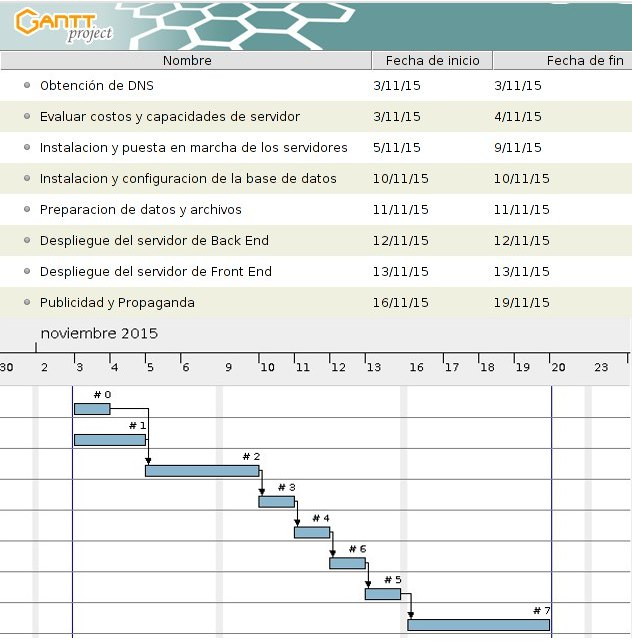
\includegraphics[width=.8\textwidth]{img/gantt_implementacion2}
	\caption{Gantt para la implementación del sistema}
	\label{gantt_implementacion2}
\end{figure}


\begin{comment}
http://velneo.es/cual-es-la-mejor-forma-de-vender-software-a-empresas-de-un-sector-especializado/
http://velneo.es/como-vender-programas-de-software/
http://velneo.es/segmentacion-de-mercado-en-software/
http://une-senn.tripod.com/new_page_3.htm
http://asistemgrp5.weebly.com/plan-de-conversioacuten.html
Método de conversión o implementación: directa, en paralelo, piloto, pruebas de versiones

Actividades: como hacer la publicidad, la promoción, como linquearlo, capacitación pilóto,  migracion de base de datos, configuración y diseño de red,
______________________________________________________________
Método de conversión del sistema, metodos, actividades y justificaciones. Siempre hay un sistema del que partimos, siempre hay una conversión de lo antiguo a lo actual. Directa, en paralelo, piloto.
Capacitación puede ser. Nuestro desafío es que la gente está muy encasillada en como se maneja con la salud, tenemos que ver como se lo vamos a hacer entrar. Antes la gente guardaba sus documentos de salud en un armario.
\end{comment}